% !TEX TS-program = pdflatex
% !TEX encoding = UTF-8 Unicode

% This is a simple template for a LaTeX document using the "article" class.
% See "book", "report", "letter" for other types of document.

\documentclass[10pt]{article} % use larger type; default would be 10pt

\usepackage[utf8]{inputenc} % set input encoding (not needed with XeLaTeX)

%%% Examples of Article customizations
% These packages are optional, depending whether you want the features they provide.
% See the LaTeX Companion or other references for full information.

%%% PAGE DIMENSIONS
\usepackage{geometry} % to change the page dimensions
\geometry{a4paper} % or letterpaper (US) or a5paper or....
\geometry{margin=1.3in} % for example, change the margins to 2 inches all round
% \geometry{landscape} % set up the page for landscape
%   read geometry.pdf for detailed page layout information

\usepackage{graphicx} % support the \includegraphics command and options

% \usepackage[parfill]{parskip} % Activate to begin paragraphs with an empty line rather than an indent

%%% PACKAGES
\usepackage{booktabs} % for much better looking tables
\usepackage{array} % for better arrays (eg matrices) in maths
\usepackage{paralist} % very flexible & customisable lists (eg. enumerate/itemize, etc.)
\usepackage{verbatim} % adds environment for commenting out blocks of text & for better verbatim
\usepackage{subfig} % make it possible to include more than one captioned figure/table in a single float
\usepackage{authblk} % allows for multiple authors and affiliations
\usepackage{amsmath} % for \text{} command
\usepackage{makecell, siunitx} % allows table headers to be two lines
\usepackage{graphicx} % for including images in document
\graphicspath{ {images/} } % image file path
\usepackage{verbatim} % for comments
\linespread{1.3} % changes line spacing to 1.5 line spacing

\usepackage{titlesec} % for changing section font sizes
\titleformat*{\section}{\large\bfseries}
\titleformat*{\subsection}{\normalsize\bfseries}
\titleformat*{\subsubsection}{\large\bfseries}
\titleformat*{\paragraph}{\large\bfseries}
\titleformat*{\subparagraph}{\large\bfseries}

% These packages are all incorporated in the memoir class to one degree or another...

%%% HEADERS & FOOTERS
\usepackage{fancyhdr} % This should be set AFTER setting up the page geometry
\pagestyle{fancy} % options: empty , plain , fancy
\renewcommand{\headrulewidth}{0pt} % customise the layout...
\lhead{}\chead{}\rhead{}
\lfoot{}\cfoot{\thepage}\rfoot{}

%%% SECTION TITLE APPEARANCE
%\usepackage{sectsty}
%\allsectionsfont{\sffamily\mdseries\upshape} % (See the fntguide.pdf for font help)
% (This matches ConTeXt defaults)

%%% ToC (table of contents) APPEARANCE
\usepackage[nottoc,notlof,notlot]{tocbibind} % Put the bibliography in the ToC
\usepackage[titles,subfigure]{tocloft} % Alter the style of the Table of Contents
\renewcommand{\cftsecfont}{\rmfamily\mdseries\upshape}
\renewcommand{\cftsecpagefont}{\rmfamily\mdseries\upshape} % No bold!

%%% END Article customizations

%%% The "real" document content comes below...

\title{\Large \vspace{-3.5cm} Using Spectrophotometry to Determine the Equilibrium Constant, $K_a$, and p$Ka$ of an Acid-Base Titration Indicator}
\author[*]{Hunter Ducharme}
\author[**]{Martha Priestly}
\author[**]{Brianna Hill}
\affil[*]{Primary author}
\affil[**]{Lab partners}
\date{} % Activate to display a given date or no date (if empty),
         % otherwise the current date is printed 

\begin{document}
\maketitle
\section{Introduction}

Products and reactants do not stop forming when a reversible chemical reaction reaches equilibrium. Rather, the rate at which reactants create products $k_f$ and the rate at which products create reactants $k_r$ are equal and thus have zero net effect on each compound's concentration. Knowing the equilibrium constant $K_a$ is useful in evaluating the ratio between $k_f$ and $k_r$. This experiment attempted to use spectrophotometry and pH data of an acid-base titration indicator (bromothymol blue) to determine the equilibrium constant of the acid-base reaction and calculate its p$K_a$.

\section{Materials and Methods}

In order to safely and properly perform this experiment, our team utilized the following materials: (a) one 250 mL beaker to act as a waste container; (b) one 150 mL beaker for preparing the initial buffer solution; (c) three 50 mL beakers for preparing the individual bromothymol blue solutions of varying pH; (d) one 5.0 mL serological pipet for transferring solution from the 150 mL beaker to the 50 mL beakers; (e) four 1.0 cm path length cuvettes for analyzing each solution in the 50 mL beakers in the spectrometer; (f) two burets for transferring water, 1.0 M HCl, and 1.0 M NaOH to the 50 mL beakers; and lastly (g) one SpectroVis Plus spectrometer for collecting data.

\subsection{Preparing the Spectrophotometric Samples}
First, three phosphate buffer solutions were prepared containing equal concentrations of the acid-base titration indicator bromothymol blue (HBB). A 150mL beaker was filled with 50mL of phosphate buffer solution, the pH of the buffer solution was recorded, then 20 drops of a 0.04\% HBB solution was added. This primary solution was then transfered to three separate 50mL beakers in 5.0mL quantities, where each beaker then recieved either 1.00 mL of 1.0 M HCl (hydrogen chloride), 1.00mL of 1.0 M NaOH (sodium hydroxide), or 1.00 mL of distilled water; these beakers were then labeled "yellow", "blue", and "green" respectively. Lastly, three cuvettes were filled with the three different solutions in the 50mL beakers resulting in a cuvette for each "yellow", "blue", and "green" solution.

\subsection{Collecting the Spectrophotometric Data}
The spectrometer was connected to the computer via USB, the software, Logger \textit{Pro}, was started and the experiment file "Equilibrium" from eCampus was opened. The software was then calibrated using a cuvette filled with distilled water, making sure the clear side of the cuvette faced the white arrow on the spectrophotometer. After calibration, three total trials were ran for the three solutions ("yellow", "blue", and "green") in the 400-700 nm wavelength range. Each cuvette was placed in the spectrometer with proper orientation (the clear side facing the white arrow) and the spectromter was allowed to run for three seconds after clicking the "Collect" button in Logger \textit{Pro}. If a dialogue box appeared asking to delete or keep the previous trial's data, our team would click on "Store Latest Run" to keep each trial's data. Once the three different spectra was colleced on the same plot, the file was saved with a '.cmbl' extension. Lastly, the workstation was cleaned, all materials were emptied and washed, and all waste was poured into the designated waste container. 

\subsection{Data Analysis}
Using the .cmbl file containing the three different spectra, a graph was produced containing the absorbance vs. wavelength plots for each sample. The maximum wavelength $\lambda_{\text{max}}$ was recorded from the graphs for bromothymol blue (HBB) and bromothymol blue anion ($\text{BB}^-$). For each $\lambda_{\text{max}}$ found, the absorption of each solution was recorded using the data table in the left-hand pane of Logger \textit{pro}. Any existing isobestic points were found and recorded using the same procedure as the last step. Lastly, the absorption for each sample was found at the wavelength 616 nm using the data table in the left-hand pane of Logger \textit{Pro}. 

\section{Results and Discussion}

\subsection{Data Summary}
For section 2.2, we found the pH of the phosphate buffer solution to be 6.76. For section 2.4, we found the $\lambda_{\text{max}}$ for HBB to be 433.4 nm, and the $\lambda_{\text{max}}$ for $\text{BB}^-$ to be 614.4 nm. We found an isobestic point at the coordinate (489.0, 0.0515) corresponding to an absorbance of a wavelength of 489 nm and an absorbance of 0.0515. The absorption values in the table below are based on the cleanliness of the cuvettes placed in the spectrometer. If the cuvettes were dirty when being placed in the spectrometer, it would hinder the light from passing through and the spectrometer would record a lesser value of absorbance. This would reduce the $K_a$ value because the absorption values would be less.

\begin{table}[h]
\centering
\begin{tabular}{ccc}
                & \thead{Absorbance, $\lambda_{\text{max}}$ for Acidic Form, \\ HBB (nm)} & \thead{Absorbance, $\lambda_{\text{max}}$ for Basic Form, \\ $\text{BB}^-$ (nm)} \\ \hline
Yellow Solution & 0.1193                                                  & -0.009947                                                        \\
Green Solution  & 0.1087                                                  & 0.08393                                                          \\
Blue Solution   & 0.03086                                                 & 0.3331                                                           \\ 
\end{tabular}
\caption{The absorbance of each solution for the $\lambda_{\text{max}}$ of both HBB and $\text{BB}^-$.}
\end{table}

\begin{figure}[h]
    \centering
    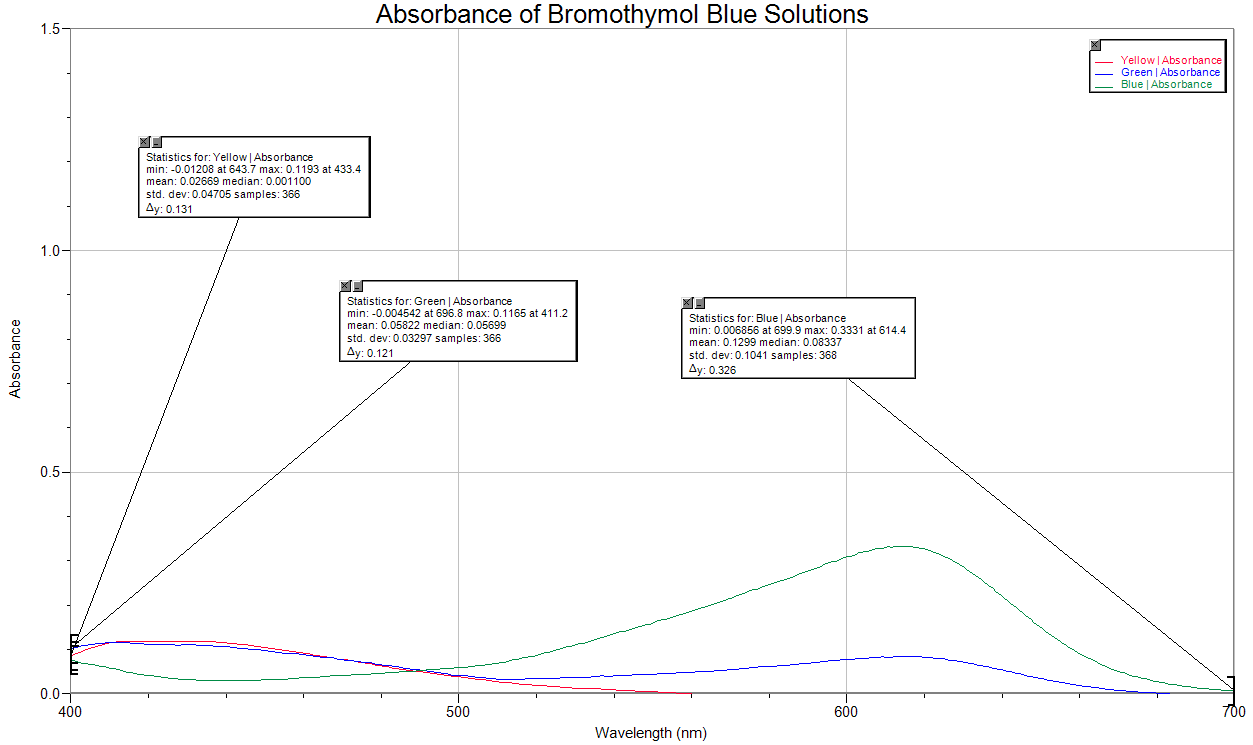
\includegraphics[width=.72\textwidth]{spectra_graph}
    \caption{The absorbance vs. wavelength plots for each solution "yellow", "blue", and "green".}
    \label{fig:mesh1}
\end{figure}

%% ONLY REASON WHY ALL EQUATIONS ARE IN-LINE IS BECAUSE MY DUMBASS CHEM 112 PROFESSOR HAS A 3 PAGE LIMIT!
\subsection{Data Analysis}
In order to calculate the equilibrium constanant $K_a$ and p$K_a$, it is necessary to first calculate the [H$_3$O$^+$] of the green solution: $\text{[H$_3$O$^+$]} = 10^{-\text{pH}} = 10^{6.76} \approx 1.738 \cdot 10^{-7}$. This can then be used to calculate $K_a$: $K_a = \text{[H$_3$O$^+$]}_{\text{green}} \cdot \left(\frac{\text{A}^{g}_{616}}{\text{A}^{B}_{616} - \text{A}^{g}_{616}} \right) = \left(1.738 \cdot 10^{-7} \right) \cdot \left( \frac{0.08373}{0.3326 - 0.08373} \right) \approx 5.862 \cdot 10^{-8}$. Next, we can find p$K_a$: $\text{p}K_a = -\text{log}(K_a) = -\text{log}(5.862 \cdot 10^{-8}) \approx 7.232$. Lastly, using literature values of $1.120\cdot10^{-7}$ for $K_a$ and $7.232$ for p$K_a$ \cite{Klotz},we can compute the percentage difference: $\text{\% diff } K_a = \frac{\lvert1.120\cdot10^{-7} - 5.862\cdot10^{-8}\lvert}{1.120\cdot10^{-7}}\cdot 100 \approx 47.66$\%; $\text{\% diff p}K_a = \frac{\lvert 6.950 - 7.232\lvert}{6.950}\cdot 100 \approx 4.058$\%.

This method of determing the equilibrium constant only works if one reaction is happening. If there was no isobestic point then that would indicate that bromothymol blue would be involved in another reaction, which would thus invalidate this method of determining the equilibrium constant. In addition, this method would work for other acid/base indicators such as thymol blue, cresol red, and phenolphthalein. The only difference is other acid/base indicators have different pH activation levels and that must be accounted for. For example, during acidic conditions, the concentration of phenolphthalein anions is too low for the magenta color to be observed, so this acid/base indicator could only work in alkaline conditions.  

A few possible sources of errors include (a) not being precise with the amount of solution being put into beakers in section 2.2, (b) accidently contaminating one solution with another with a couple of drops, (c) not properly cleaning the cuvettes when placing them into the spectrometer, (d) not cleaning the lens on the spectrometer where the light is shot out of, and (e) having contaminates inside of the solutions such as small dirt particles or other things that would hinder the passage of light through the solution.

\section{Conclusion}
Computing the equilibrium constant $K_a$ and p$K_a$ of the acid-base titration indicator bromothymol blue with spectrophotometry methods was fairly successful. Our results for $K_a$ and p$K_a$ had a 47.66\% and 4.058\% error compared to the current literature values for these parameters.


\newpage 
\bibliography{technical_abstract} 
\bibliographystyle{apalike}


\end{document}
